\section{Background}\label{sec:background}

\subsection{Mixed Integer Linear Programming (MILP) Problems}\label{subsec:mixed-integer-linear-programming-(milp)-problems}
These problems are linear optimization problems where some of the decision variables are integers, and some are continuous.
It is possible to formulate MILP problems as follows:

\begin{equation*}
    \begin{aligned}
        \text{minimize} \quad & \textbf{c}^T \textbf{x} \\
        \text{s.t.} \quad & \textbf{A}\textbf{x} \leq \textbf{b} \\
        & \textbf{x} \in \mathbb{Z}^p \times \mathbb{R}^{n-p}\\
    \end{aligned}\label{eq:equation}
\end{equation*}


where \textbf{c} \begin{math} \in \mathbb{R}^n \end{math} represents the objective coefficient vector, \textbf{A} \begin{math} \in \mathbb{R}^{mxn} \end{math} represents the constraint coefficient matrix, \textbf{b} \begin{math} \in \mathbb{R}^m \end{math} represents the right-hand-side vector, and  p \begin{math} \leq \end{math} n indicates the number of integer variables.
MILP problems are usually solved by Branch \& Bound algorithm.


\subsection{The LP Relaxation of a MILP Problem}\label{subsec:the-lp-relaxation-of-a-milp-problem}
LP Relaxation of a MILP problem is the problem obtained by ignoring the integrality conditions on the variables in the MILP problem as follows:

\begin{equation*}
    \begin{aligned}
        \text{minimize} \quad & \textbf{c}^T \textbf{x} \\
        \text{s.t.} \quad & \textbf{A}\textbf{x} \leq \textbf{b} \\
        & \textbf{x} \in \mathbb{R}^{n}\\
    \end{aligned}\label{eq:equation2}
\end{equation*}


It is possible to solve this form of the problem using Linear Programming (LP) techniques such as Simplex algorithm.


\subsection{Bipartite Graph Representation of a MILP Problem}
\label{sec:bipartite_graph_representation}
To employ GNN techniques, such as GCNN and GAT, in tackling Combinatorial Optimization problems, these problems need to be represented as graphs.
Combinatorial Optimization problems can be represented as bipartite graphs.
The nodes on the left side of the bipartite graph represent the constraints in the MILP problem, with each constraint corresponding to a node.
The nodes on the right side of the bipartite graph represent the variables in the MILP problem, with each variable corresponding to a node.
If a variable is part of a constraint, there is an undirected edge between the corresponding nodes.
The coefficient of the variable in the constraint is a feature of the corresponding edge.
Figure~\ref{fig:biparite-graph} illustrates the bipartite graph representation of a MILP problem with 3 variables and 2 constraints.

\begin{figure}[htb!]
    \centering
    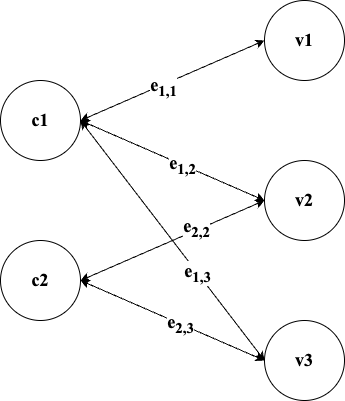
\includegraphics[width=0.25\textwidth]{figures/Bipartite Graph.drawio}
    \caption{Bipartite graph representation of a MILP problem with n = 3 variables and m = 2 constraints. If a variable is part of a constraint, there is an undirected edge between the corresponding nodes.}
    \label{fig:biparite-graph}
\end{figure}

\subsection{Branch \& Bound Algorithm}\label{subsec:branch-bound-algorithm}
In the Branch \& Bound algorithm, first, the LP relaxation of the MILP problem is solved with Linear Programming methods.
If the optimal solution satisfies the integrality conditions of the problem, then the optimal solution of the original problem is reached.
If the optimal solution does not satisfy the integrality conditions of the problem, the optimal objective value of the LP relaxation is set as the lower bound, and $\infty$ is set as the upper bound for the optimal objective value of the original problem (for minimization problems).
Variables in the solution that do not satisfy integrality conditions are candidates for branching.
A branching variable $x_i$ is selected from among the branching candidates by means of a branching strategy (such as Strong Branching).
The problem is then split into two separate sub-problems by adding the conditions $x_i \leq \lfloor x_i \rfloor$ and $x_i \geq \lceil x_i \rceil$ separately and two separate nodes are added to the search tree.
One of the non-investigated nodes is selected, and the corresponding LP relaxation is solved.
Subsequently, the following process is executed:

\begin{itemize}
  \item If there is no feasible solution for the LP relaxation of the problem at the relevant node, the node is pruned and not further investigated (\textit{pruned by infeasibility}).
  \item If there is a feasible solution for the LP relaxation of the problem at the relevant node, the objective value of optimal solution is compared with the upper bound of the optimal objective value of the original problem:
  \begin{itemize}
    \item If the optimal value of the LP relaxation is greater than the upper bound of the optimal value of the original problem, the node is pruned and not further investigated (\textit{pruned by bound}).
    \item If the optimal value of the LP relaxation is smaller than the upper bound of the optimal value of the original problem,
      \begin{itemize}
          \item If solution satisfies the integrality conditions of the original problem, then the upper bound is updated as the optimal value of the LP relaxation.
          This node is pruned and not further investigated (\textit{pruned by optimality}).
          \item If solution does not satisfy the integrality conditions of the original problem, then one of the variables that do not satisfy the integrality conditions in the solution is selected by help of a branching strategy, and branching is performed.
          \end{itemize}
  \end{itemize}
\end{itemize}

When upper and lower bounds are equal or when there is no non-investigated node, then the algorithm reached the optimal solution.
The best feasible solution is the optimal solution.
Figure~\ref{fig:branch-bound} illustrates the flow of the Branch \& Bound algorithm.

\begin{figure}[htb!]
    \centering
    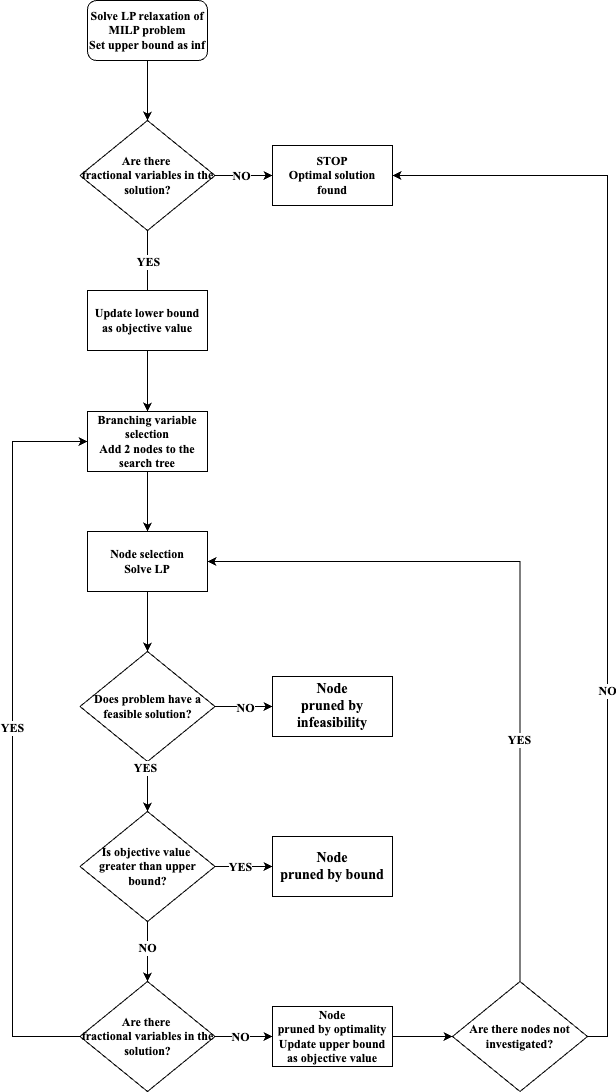
\includegraphics[width=0.5\textwidth]{figures/Branch and Bound.drawio}
    \caption{Branch \& Bound algorithm steps for minimization problems.}
    \label{fig:branch-bound}
\end{figure}


\subsection{Strong Branching}\label{subsec:strong-branching}
In each iteration of the Branch \& Bound algorithm, two important choices that affect the algorithm's performance are made: node selection and branching variable selection.
Specifically, selecting a better branching variable positively influences the length of the search tree generated by the algorithm.
Therefore, researchers have proposed various strategies in the literature regarding the selection of the branching variable.
Among these strategies, the one that keeps the search tree length shortest is Strong Branching.
In the Strong Branching strategy, a branching simulation is conducted for each variable that can be a branching variable.
For each variable, two new nodes are added to the problem hypothetically, and the two problems are solved separately.
The changes in the objective values obtained in the two problems are used to create a Strong Branching score for each variable.
The variable with the highest Strong Branching score is selected as the branching variable.
Because the Strong Branching strategy simulates the branching decision for all candidate variables, it is generally successful in selecting the better branching variable and keeping the search tree short.
However, since it solves the linear programming problem twice for each candidate variable, the Strong Branching strategy is very time-consuming.

Consider a node N with LP value $z^*$, the two children $N_i^-$ and $N_i^+$ nodes, resulting from branching on $i$ downwards and upwards, have (feasible) LP values $z_i^-$ and $z_i^+$, respectively.
The changes in objective value are then $\Delta_i^- = z_i^- - z^* $  and $\Delta_i^+ = z_i^+ - z^* $.
Then Strong Branching score of variable $i$ is calculated as following: $$S_i = score (\max \{\Delta_i^-, \epsilon\}, \max \{\Delta_i^+, \epsilon\}) $$
where $\epsilon$ is a small constant (e.g. $10^-6$). A product is commonly utilized for scoring purposes such as $score(a, b) = a x b$.


\subsection{Neural Networks (NNs)}\label{subsec:neural-networks-(nns)}
A neural network is a machine learning algorithm inspired by the structure and function of the human brain.
It is particularly effective at addressing complex problems, such as image recognition and natural language processing, which are challenging for traditional algorithms to solve.


Neural networks are composed of interconnected units known as neurons, which are organized into layers.
Each neuron takes input from other neurons, processes this information, and passes the result to subsequent neurons.
The connections between neurons are weighted, indicating the strength of the connection.
During the training process, the network adjusts these weights to enhance its accuracy for a given task.
This capability to learn and adapt allows neural networks to identify patterns and make predictions, making them widely used in fields like image recognition, natural language processing, and machine translation.


A fully connected multi-layer perceptron (MLP) is a type of neural network where each neuron in one layer is connected to every neuron in the subsequent layer as can be seen in Figure~\ref{fig:mlp}.

\begin{figure}[htb!]
    \centering
    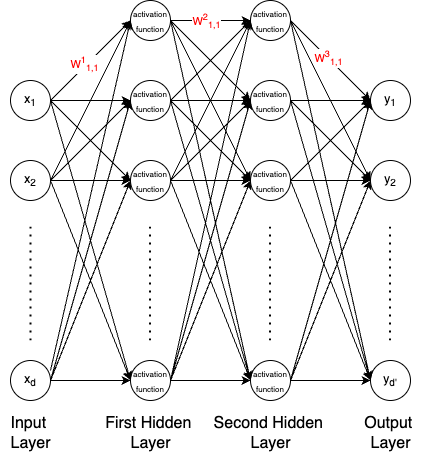
\includegraphics[width=0.5\textwidth]{figures/MLP}
    \caption{A fully connected Multi-Layer Perceptron (MLP) which maps d dimensional node feature vector to d’ dimensional node embedding vector with a nonlinear activation function such as ReLU and learnable weight matrices ($W^1$, $W^2$ and $W^3$).}
    \label{fig:mlp}
\end{figure}


\subsection{Graph Neural Networks (GNNs)}\label{subsec:graph-neural-networks-(gnns)}
A graph is a type of data structure consisting of nodes and edges between those nodes.
A node can represent an individual, an object, a document, a molecule, etc., while the edges represent the relationships between the nodes.
Graphs are particularly useful for depicting interactions and relationships between objects.
They are frequently used in fields such as social network analysis, recommendation systems, and drug discovery.


To further describe each node, edge or the entire graph, we can store information in each of these pieces of the graph as node features, edge features and graph features as can be seen in Figure~\ref{fig:graph}.

\begin{figure}[htb!]
    \centering
    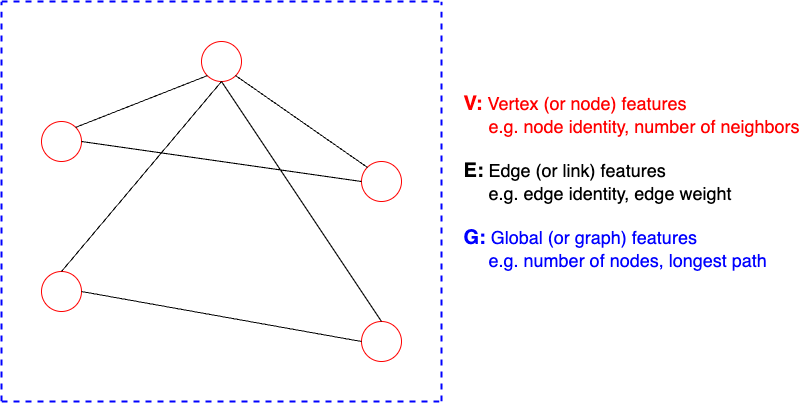
\includegraphics[width=0.5\textwidth]{figures/Graph.drawio}
    \caption{Graph and three types of features, node features, edge features and graph features.}
    \label{fig:graph}
\end{figure}


The machine learning community has focused on addressing problems that can be represented as graph-structured data.
Broadly, these problems are categorized into three primary learning tasks: graph-level learning, node-level learning, and edge-level learning:


\begin{itemize}
  \item Graph-level learning aims to predict a property or characteristic of the entire graph.
  For instance, given a molecular graph, one can predict whether the molecule will bind to a receptor associated with a specific disease.
  \item Node-level learning focuses on predicting a property or attribute of individual nodes within a graph.
  For example, in a citation network, it is possible to predict the research field of a particular paper, represented as a node in the graph.
  \item Edge-level learning seeks to predict a property or attribute of the edges within the graph.
  For instance, using the graph representation, one could predict the nature of the relationship (an edge) between objects in an image.
\end{itemize}


To perform these learning tasks, the machine learning community has leveraged node features, edge features, graph features, and connectivity data, often employing Graph Neural Networks (GNNs).
A GNN is a trainable framework that transforms node, edge, and graph features using nonlinear activation functions and learnable weight matrices.
Training GNNs involves feedforward propagation and backpropagation techniques.
During the training process, the network adjusts its weights based on the examples in the training dataset to minimize a specified loss function.
As can be seen in Figure~\ref{fig:gnn}, within a GNN layer, while the graph structure and connectivity remain unchanged, node, edge, and graph embeddings are updated by a differentiable model such as fully connected Multi-Layer Perceptron (MLP).


\begin{figure}[htb!]
    \centering
    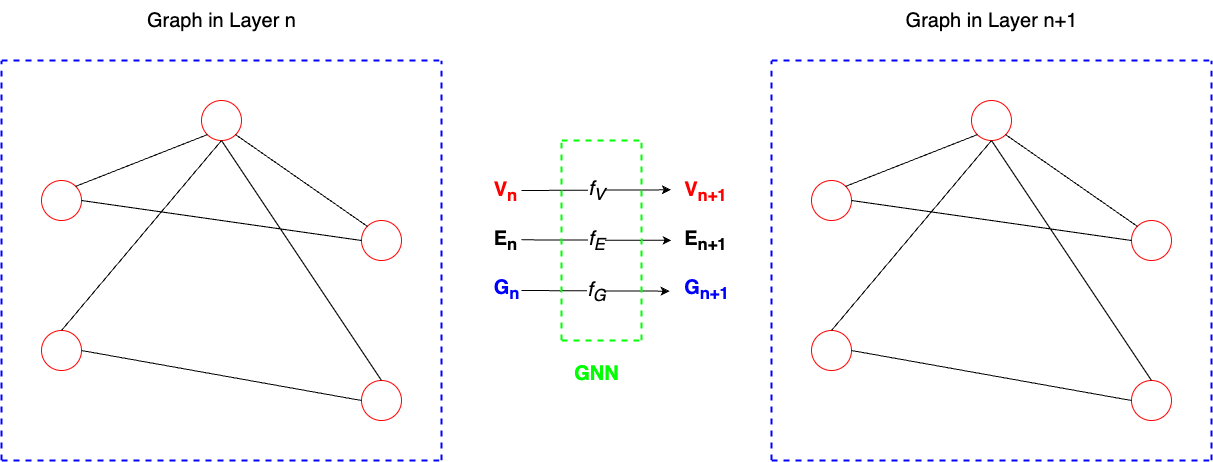
\includegraphics[width=0.5\textwidth]{figures/GNN}
    \caption{A single layer of GNN.
    Node, edge and graph features gets updated by a differentiable model ($f_V, f_E, f_G$) such as fully connected Multi-Layer Perceptron (MLP) with preserving graph structure and connectivity.}
    \label{fig:gnn}
\end{figure}


\subsubsection{Neural Message Passing}\label{subsec:neural-message-passing}
Connectivity (or adjacency) is an important concept of graph structured data.
Neural Message Passing allows GNNs to utilize connectivity information.
In Neural Message Passing, nodes exchange information with their neighboring nodes and aggregate that information to update their own representations.
This enables GNNs to capture both the structural information of the graph and the features associated with each node.
In Neural Message Passing, first, computation graph for each node is constructed as can be seen in Figure~\ref{fig:message-passing}.
Then in each GNN layer, messages from neighboring nodes are collected and aggregated.


\begin{figure}[htb!]
    \centering
    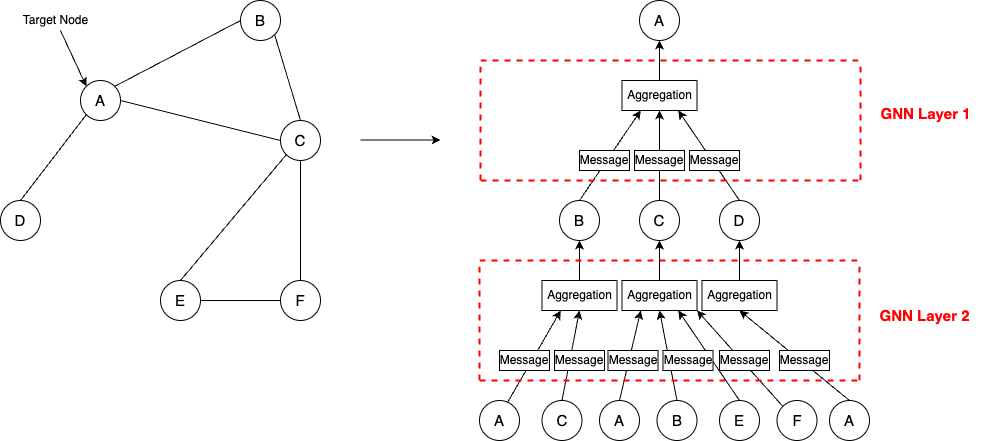
\includegraphics[width=0.5\textwidth]{figures/Message Passing.drawio}
    \caption{Computation graph of node A based on its 2-hop neighborhood.
    A single GNN layer collects messages from neighboring nodes and aggregate them.}
    \label{fig:message-passing}
\end{figure}


Neural Message Passing networks can be described mathematically as following: $$x_i^{(n+1)} = \gamma^{(n+1)}(x_i^n, \bigoplus \phi^{(n+1)}(x_i^n, x_j^n, e_{j,i}))$$
where $j \in N(i)$, $\bigoplus$ denotes a differentiable, permutation invariant aggregation function, e.g., sum, mean or max, and $\gamma$ denotes differentiable update function, $\phi$ denotes differentiable message function such as MLPs (Multi-Layer Perceptrons).


\subsubsection{Graph Convolutional Neural Networks (GCNNs)}\label{subsec:graph-convolutional-neural-networks-(gcnns)}
Graph Convolutional Neural Network (GCNN) is a special type of neural message passing network.
A significant portion of GNN applications is composed of GCNNs. The GCNN layer is mathematically defined as following: $$x_i^{(n+1)} = \textcolor{blue}{\sigma}(\sum_{j \in N(i) \cup {i}} \textcolor{red}{\frac{1}{|N(i)|}}(\textcolor{red}{W^T}x_j^n)$$


In GCNN, sum is preferred as aggregation function ($\bigoplus$ in neural message passing formulation), \textcolor{red}{red} operation denotes message function ($\phi$ in neural message passing formulation), \textcolor{blue}{blue} operation denotes update function ($\gamma$ in neural message passing formulation).
Note that $\frac{1}{|N(i)|}$ is the weighting factor (importance) of node $j$’s message to node $i$.
Therefore, all neighbors $j \in N(i)$ are equally important to node $i$.


\subsubsection{Graph Attention Networks (GATs)}\label{subsec:graph-attention-networks-(gats)}
Graph Attention Network (GAT) is another type of neural message passing network. The GAT layer is mathematically defined as following: $$x_i^{(n+1)} = \textcolor{blue}{\sigma}(\sum_{j \in N(i)} \textcolor{red}{\alpha_{ij}}(\textcolor{red}{W^{n+1}}x_j^n)$$


In GAT, sum is preferred as aggregation function ($\bigoplus$ in neural message passing formulation), \textcolor{red}{red} operation denotes message function ($\phi$  in neural message passing formulation), \textcolor{blue}{blue} operation denotes update function ($\gamma$ in neural message passing formulation).

Unlike traditional GNNs, which rely on fixed aggregation schemes (e.g., averaging or summing), GAT dynamically assigns different weights to neighboring nodes based on their importance, allowing the model to focus more on relevant parts of the graph.
Note that $\alpha_{ij}$ are the attention weights.
Because not all neighbors of a node hold equal significance, attention $\alpha_{ij}$ emphasizes the most relevant portions of the input data while diminishing the influence of less important parts. $\alpha_{ij}$ are computed in 2 steps:


\begin{itemize}
  \item Step 1: Let $f$ is an attention mechanism and it computes attention coefficients $e_{ij}$ across pairs of nodes $i$, $j$ based on their messages: $$ e_{ij} = f(W^{(n+1)}x_j^n, W^{(n+1)}x_i^n) $$ where $e_{ij}$ indicates the importance of node $j$’s messages to node $i$.
  \item Step 2: Normalize $e_{ij}$ into the final attention weight $\alpha_{ij}$ by using the SoftMax function, so that $\sum_{j \in N(i)} \alpha_{ij} = 1 $. $$ \alpha_{ij} = \frac{e^{e_{ij}}}{\sum_{k \in N(i)} e^{e_{ik}}} $$
\end{itemize}


Multi-head attention is an extension of the attention mechanism that uses multiple independent attention mechanisms (or "heads") in parallel to learn different aspects of the graph structure and node relationships.
By combining the outputs from these attention heads, the model achieves a richer and more robust representation of the graph data.
In Multi-Head Attention method, multiple attention scores are created with different attention mechanisms, $ f^1, f^2, .... , f^N $ represents different attention functions: $$ e_{ij}^1 = f^1(W^{(n+1)}x_j^n, W^{(n+1)}x_i^n), \alpha_{ij}^1 = \frac{e^{e_{ij}^1}}{\sum_{k \in N(i)} e^{e_{ik}^1}} $$ $$ e_{ij}^2 = f^2(W^{(n+1)}x_j^n, W^{(n+1)}x_i^n), \alpha_{ij}^2 = \frac{e^{e_{ij}^2}}{\sum_{k \in N(i)} e^{e_{ik}^2}} $$ $$ ...... $$ $$ e_{ij}^N = f^N(W^{(n+1)}x_j^n, W^{(n+1)}x_i^n), \alpha_{ij}^N = \frac{e^{e_{ij}^N}}{\sum_{k \in N(i)} e^{e_{ik}^N}} $$


Then outputs are aggregated by concatenation or summation as can be seen in Figure~\ref{fig:mh-gat}: $$ x_i^{(n+1)} = AGG(\sigma(\sum_{j \in N(i)} \textcolor{red}{\alpha_{ij}^1}(W^{(n+1)}x_j^n), \sigma(\sum_{j \in N(i)} \textcolor{red}{\alpha_{ij}^2}(W^{(n+1)}x_j^n), . ,$$ $$ \sigma(\sum_{j \in N(i)} \textcolor{red}{\alpha_{ij}^N}(W^{(n+1)}x_j^n)) $$
.
\begin{figure}[htb!]
    \centering
    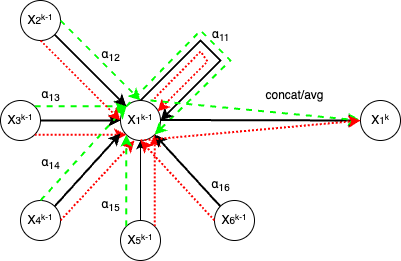
\includegraphics[width=0.5\textwidth]{figures/MH GAT.drawio}
    \caption{Multi Head Graph Attention Network with 3 attention heads. Various arrow styles and colors represent separate attention computations.}
    \label{fig:mh-gat}
\end{figure}


\subsection{Rectified Linear Unit (ReLU)}\label{subsec:rectified-linear-unit-(relu)}
Rectified Linear Unit (ReLU) are a class of activation functions characterized by linear behavior in the positive domain and a value of zero in the negative domain.
This function can be written as follows: $$ f(x) = \max \{0, x\}  $$


\subsection{SoftMax}\label{subsec:softmax}
Softmax is a widely used activation function in neural networks, particularly as the final activation layer.
Its primary role is to normalize the network's outputs into a probability distribution across the predicted output classes.
This function can be written as follows: $$ f(x_i) = \frac{e^{x^{i}}}{\sum_{j = 1}^{n} e^{x{j}}} $$


\subsection{Cross Entropy Loss}\label{subsec:cross-entropy-loss}\
Cross-entropy, also known as logarithmic loss or log loss, is a popular loss function used to measure the performance of a classification model.
This loss function can be written as follows: $$ H = - \sum p(x)logq(x) $$ where $p(x)$ is true probability distribution and $q(x)$ is the model’s predicted probability distribution.